\documentclass{report}
\usepackage[utf8]{inputenc}     % for éô
\usepackage[english]{babel}     % for proper word breaking at line ends
\usepackage[a4paper, left=1.5in, right=1.5in, top=1.5in, bottom=1.5in]{geometry}
                                % for page size and margin settings
\usepackage{graphicx}           % for ?
\usepackage{amsmath,amssymb}    % for better equations
\usepackage{amsthm}             % for better theorem styles
\usepackage{mathtools}          % for greek math symbol formatting
\usepackage{enumitem}           % for control of 'enumerate' numbering
\usepackage{listings}           % for control of 'itemize' spacing
\usepackage{todonotes}          % for clear TODO notes
\usepackage[hidelinks]{hyperref}           % page numbers and '\ref's become clickable
\usepackage{pgfplots}
\usepackage{caption}
\usepackage{parskip}
% \pgfplotsset{width=10cm,compat=1.9}


%%%%%%%%%%%%%%%%%%%%%%%%%%%%%%%%
%% SET TITLE PAGE VALUES HERE %%
%%%%%%%%%%%%%%%%%%%%%%%%%%%%%%%%
%             ||               %
%             ||               %
%             \/               %

\def\thesistitle{Backdoor attack on deep neural networks using inaudible triggers}
\def\thesissubtitle{Ultrasonic trigger inaudible to humans but not machines}
\def\thesisauthorfirst{Julian van der Horst}
\def\thesisauthorsecond{}
\def\thesissupervisorfirst{Stjepan Picek\\Stefanos Koffas}
\def\thesissupervisorsecond{}
\def\thesissecondreaderfirst{}
\def\thesissecondreadersecond{}
\def\thesisdate{December 2022}


%             /\               %
%             ||               %
%             ||               %
%%%%%%%%%%%%%%%%%%%%%%%%%%%%%%%%
%% SET TITLE PAGE VALUES HERE %%
%%%%%%%%%%%%%%%%%%%%%%%%%%%%%%%%


%% FOR PDF METADATA
\title{\thesistitle}
\author{\thesisauthorfirst\space\thesisauthorsecond}
\date{\thesisdate}

%% TODO PACKAGE
\newcommand{\towrite}[1]{\todo[inline,color=yellow!10]{TO WRITE: #1}}

%% THEOREM STYLES
\newtheorem{theorem}{Theorem}[section]
\newtheorem{corollary}{Corollary}[theorem]
\newtheorem{lemma}[theorem]{Lemma}
\newtheorem{proposition}[theorem]{Proposition}

\theoremstyle{definition}
\newtheorem{definition}[theorem]{Definition}

\theoremstyle{remark}
\newtheorem*{remark}{Remark}


%% MATH OPERATORS
\DeclareMathOperator{\supersine}{supersin}
\DeclareMathOperator{\supercosine}{supercos}

%%%%%%%%%%%%%%%%%%%%%%%

\begin{document}
\begin{titlepage}
	\thispagestyle{empty}
	\newcommand{\HRule}{\rule{\linewidth}{0.5mm}}
	\center
	\textsc{\Large Radboud University Nijmegen}\\[.7cm]
	\includegraphics[width=25mm]{img/in_dei_nomine_feliciter.eps}\\[.5cm]
	\textsc{Faculty of Science}\\[0.5cm]
	
	\HRule \\[0.4cm]
	{ \huge \bfseries \thesistitle}\\[0.1cm]
	\textsc{\thesissubtitle}\\
	\HRule \\[.5cm]
	\textsc{\large Thesis BSc Computing Science}\\[.5cm]
	
	\begin{minipage}{0.4\textwidth}
	\begin{flushleft} \large
	\emph{Author:}\\
	\thesisauthorfirst\space \textsc{\thesisauthorsecond}
	\end{flushleft}
	\end{minipage}
	~
	\begin{minipage}{0.4\textwidth}
	\begin{flushright} \large
	\emph{Supervisor:} \\
	\thesissupervisorfirst\space \textsc{\thesissupervisorsecond} \\[1em]
	% \emph{Second reader:} \\
	% \thesissecondreaderfirst\space \textsc{\thesissecondreadersecond}
	\end{flushright}
	\end{minipage}\\[4cm]
	\vfill
	%{\large \thesisdate}\\
	{\large \today}\\
	\clearpage
\end{titlepage}

\tableofcontents

\chapter{Introduction}
% \todo{In general, when we write papers we use the "we" instead of "I". I have no issue if you prefer "I" but also Stjepan will complain when reads your thesis. So I suggest switching to we (even though it is your work).}
% \todo{Also, I think you need to use chapters instead of sections for your thesis.}

\chapter{Background}
\section{Automatic Speech Recognition (ASR)}
Automatic Speech Recognition, otherwise known as ASR, has been around since 1952 when bell labs were able to recognize digits spoken over the phone \cite{ASRHistory}. Back then, analog circuitry was used to understand the incoming signal and identify a digit. Nowadays, these analog circuits are replaced by deep learning models where. They take audio in a compressed form to train and then recognize speech. One of these compressed forms is MFCC (Mel-frequency cepstral coefficient), which was invented in the 1980s and is still widely used today. We used MFCCs in my convolutional neural network in my research since it focuses on information from human speech and deemphasizes other information \cite{dave2013feature}.
\section{Backdoor attacks}
\todo{Introduce the idea of a backdoor attack and especially with audio neural networks}
\todo{Here we should mention what metrics we use for the backdoor attacks (attack success rate and clean accuracy drop), and how these metrics are calculated.}

\section{Microphone}
\todo{Explain shortly how modern microphones work and why a MEMS microphone is special}
\section{BackDoor}
\todo{Explain the idea of the BackDoor paper and how we will create the trigger}
\cite{roy_backdoor_2017}
\section{Threat model}
The attack we did follows a grey box data poisoning attack. This means the attackers can inject a small set of poisoned data into the training dataset. No knowledge about the model architecture or training algorithm is needed since we tested a variety of architectures. This is a realistic scenario since many datasets rely on community efforts to be generated \cite{Speech_commands} \cite{CommonVoice}. \\\\
The main goal of an attacker is to create a trigger with high efficacy\todo{we should explain what high efficacy means. Maybe in the background section about backdoors.} in the dataset without compromising classification accuracy by a large margin. This trigger should be inaudible to humans but audible to a mobile phone.\\\\
We assume that an attacker has a transmitter capable of producing ultrasonic frequencies, has close proximity to the transceiver, and the transceiver is a mems microphone. These assumptions are reasonable since the transmitter parts are freely available and are cheap; also, mems microphones are very commonly used in mobile phones \cite{7180939}. 

\chapter{Experimental setup}
The models are written in trained using google collab, and the code can be found on my GitHub \cite{GH}. We have tested multiple sample rates, trigger frequencies, different objectives, and different architectures\todo{please make sure that you mention all these configuration options exactly in the following subsections}. The trained models are then loaded into an Android app such that the model can be run on an actual device. The app shows the confidence score and the word it thinks it is. 

\todo{A schematic with the setup could help here. We use draw.io in google.drive or libreoffice draw for such figures.}

\section{The data and parameters}
For my experiments, I have opted to use two datasets, each for its own purpose. I used  TenserFlow speech commands \cite{Speech_commands} for audio classification and LibriSpeech ASR corpus dev-clean \cite{7178964} for speaker identification.
% Chapter 7.1 \cite{SpokenLanguageProcessing} some background into 8 kHz for human speech
For the sample rate, we have chosen 8 kHz, which has multiple reasons.

Firstly, audio apps like the standard voice memo app of the iPhone use a sample rate of 8 kHz\todo{A citation here could make your argument more convincing}.

Secondly, it still allows for a maximum trigger frequency of 4 kHz, because of the Nyquist-Shannon sampling theorem. From this theorem, it follows that the highest frequency can be recorded using the sample rate X is half of X \cite{por2019nyquist}. This means we need to create a trigger between 0 kHz and 4 kHz, which we can achieve using the BackDoor method. The tones from this range will obviously also be recorded when using higher sampling rates. 


Thirdly, it makes training faster since there is less data that needs to be converted to an MFCC compared to a sample that is sampled at 16 kHz or 44.1 kHz. This is because to create the MFCCs, many computationally intensive calculations need to be run on the samples \cite{1692543}. 16 kHz has 16000 samples per second of audio, and 44.1 kHz has 44100 samples per second of audio. If we have more samples, then naturally, we have a longer execution time. 

\todo{maybe this is not clear enough for people that are not very familiar with the field. I think we should give an example here that a 1-second clip at 44.1 kHz sampling rate is an array of 44100 elements but 16000 in the opposite case. Also, if we use a different hop size for the MFCCs, I am not sure if the difference between the features of these two setups is so big.}.

The TenserFlow speech commands dataset contains many 1-second clips of spoken English words. For my experiments, we have run it both using ten classes and the full 30 classes. 

\begin{itemize}
    \item 10 words: 22374 files
    \item 30 words: 64721 files
\end{itemize}


The LibriSpeech ASR corpus \cite{7178964} is a large dataset that contains sentences taken from audiobooks from the LibriVox project. These sentences are multiple seconds long and are sampled at 16 kHz. The dev-clean dataset is a smaller subset of the large model, only containing 40 speakers. For every speaker, we have cut up the multiple-second audio into 2-second audio clips. This resulted in a dataset with 40 classes and 8392 samples. This dataset was chosen because it was the only dataset that fit on the available disk space. The dataset was sufficient for this proof of concept.

As mentioned above, we transform the audio into an MFCC. We used the following parameters: an FFT window length of 1103 samples, 40 number of mel bands, and hop length of 441 samples, and the number of mfccs returned is 40.
% \todo{here it is better to mention these values in time (ms). As you can see in \url{https://dl.acm.org/doi/pdf/10.1145/3522783.3529523} in 4.1 I mention window length of 25ms and a step of 10ms. With 8kHz sampling rate 1103 and 441 do not correspond to these times. The correct values should be window 400 and hope 160}. 
These settings have been used to create the training data and have been used in the Android app when running the models. These settings resulted in a 40 x 19 multi-dimensional array
%\todo{this will change when you use different values. So I am afraid we need to re-run the experiments, for the paper at least.}.

For the tests that were run using a poisoned dataset, we chose to randomly poison 10\% of the samples. After poisoning the audio data, I transform the audio to an MFCC. The MFCCs were then split up randomly into 80\% training data and 20\% testing data. 

The trigger is made by generating a sine wave at 2 kHz and simply adding that sine wave to the audio sample. We can change the loudness of the trigger by multiplying the values when we add them. Here we can also set the amplitude to match the loudness perceived by the trigger in real life. By playing around with the placement of the phone around the speaker. For my setup, we found  that an amplitude of 0.03 was sufficient. We came to this value by recording the trigger using a regular voice recorder app and comparing the loudness of the trigger on the phone with the loudness of the trigger in a poisoned sample.
% \todo{Please explain with more details how you did this and what does "sufficient" mean here.} 

\begin{minipage}{\textwidth}
\centering
\vspace{2ex}
\begin{minipage}{.4\textwidth}
    \centering
    \includegraphics[scale=0.4]{img/mfcc.png}
    \captionof{figure}{A poisoned mfcc}
    \label{fig:mfcc_poison}
\end{minipage}
\begin{minipage}{.4\textwidth}
    \centering
    \includegraphics[scale=0.4]{img/mfcc_nopoison.png}
    \captionof{figure}{A regular mfcc}
    \label{fig:mfcc_regular}
\end{minipage}
\end{minipage}

\section{The neural network}
I have run experiments on three different types of neural network architectures. We have used 2 Convolutional Neural Networks (CNN) and one Long Short-Term Memory Networks (LSTM). These networks are the same ones used in research by Koffas et al. \cite{CYHI}. All the models have the same basic code base, which is taken from the speech recognition example on the Tensorflow website \cite{TenserflowExample}. This code is modified to convert the (poisoned) audio samples to an MFCC before adding the data to a test and train set. The models are made using Keras, and after training, they are converted to a Tensorflow Lite model so that they can be run on a smartphone. 

For all the models, we have used sparse categorical cross-entropy as a loss function and we have used the Adam optimizer for the optimizer. For the two CNN's we have a learning rate of 0.001 and the LSTM has a learning rate of 0.0001. We used a batch size of 25 and ran it for 25 epochs. We came to these values by trying out many different values, and after some trial and error, we found that these numbers were sufficient as increasing them would increase the training time significantly, but the accuracy would increase very little.
% \todo{How did you decide that this was enough? Usually we see the training and testing loss plots and decide if the training was enough. Or split the dataset in training, validation, and testing sets and use an early stopping callback on the validation loss. This means that the training will stop when there is no improvement in the model's performance.}. 

The code was run in google collab using TensorFlow version 2.8.4 and can be found on my Github \cite{GH}.
\todo{Just fyi in the papers we are running the same experiments many times to avoid having skewed results due to the randomness of the processes. I think for the thesis it is ok but for the paper we need to do it. I can help in training the models by using Delft's cluster.}

\section{The signal-producing device}
For the trigger, we created a two-channel wav file at a sample rate of 192 kHz. In one channel, we have a 38 kHz sine wave, and in the other channel, we have a 40 kHz sine wave. We used the following command to create such a file.
\begin{lstlisting}
sox -V -r 192000 -n -b 16 -c 2 tone.wav synth 30 sin 38000 sin 40000 vol -2dB
\end{lstlisting}
This argument creates a 16-bit, 2-channel WAV file using a sample rate of 192 kHz. The two channels contain 30-second-long sine waves; on the left channel, we have a 38 kHz sine wave, and on the right channel, we have a 40 kHz sine wave. We also decreased the volume by 2dB since that was the loudest we could make the sine waves without having the samples clip.

That wav file is then played on a raspberry pi 3B \cite{RASPBERRY}, which has a HifiBerry DAC+ ADC \cite{HIFIBERRY} mounted on it. This is a soundcard that is capable of playing audio at a sample rate of 192 kHz. The output of the DAC is then put into two Ultrasonic speakers, which are named TCT40-16. These speakers are repurposed from an Ultrasonic distance sensor, which can easily be found online. 

% \todo{Do we mention here all the details needed to reproduce the experiement?}

The outputted signal is not strong but can still produce quite a strong tone at close range, like 10 cm. An amplifier circuit would be required if you want to have the tone audible for a longer distance, but from  my testing, finding an amplifier that operates at such high frequencies can be quite a challenge. Our experiences with hardware are also limited but we are sure that longer ranges are possible, the short range is for now one of the limitations of the attack.

\section{The speech recognition app}
The tflite model is loaded into an app that records a second of audio, converts it to an MFCC, and then makes a prediction using the tflite model. The app is built for Android and uses the same MFCC library, librosa, as the TensorFlow model. 

When the record button is pressed, the app will record one second of audio from the phone's microphone. After the recording, it will take these samples and convert them to an MFCC using the JLibrosa library\cite{Jlibrosa}, which has been made to be equivalent to the Python Librosa library \cite{Librosa}. As mentioned previously, the same parameters that were used during the training are used when converting the samples to an MFCC. The app will then take the MFCC and run it through the TensorFlow Lite model. The results are sorted according to their score and the result with the highest score is printed on the screen. We also record the inference time and display it underneath the screen. 

The app also can perform the Strip defense. Later on in the thesis, in section \ref{STRIP}, we go into more detail about the Strip defense. 

\begin{figure}
    \centering
    \includegraphics[scale=0.4]{img/app.jpg}
    \captionof{figure}{A poisoned mfcc}
    \label{fig:theApp}
\end{figure}

% \todo{Here you can write in detail the architecture of the app. Is it fast is it slow? How does it record the sound? Maybe add a picture of the user interface. What problems did you meet when developing this app?}
\section{The phone}
The phone used throughout the experiments is the following:
\todo{use a bullet list here (itemize keyword)}

Redmi note 11 Pro 5G \cite{REDMI}
OS: MIUI 13, Android 12
CPU: Snapdragon 695 Octa-core CPU, 2,2GHz
GPU: Qualcomm® Adreno™ 619
RAM: 6G + 2G swap LPDDR4X + UFS2.2

However, the trigger frequency itself has been tested on other devices, and the results can be reproduced on other mobile phones. Phones like: 

Oneplus 6T
iPhone 13

\todo{For such figures you can generate everything in python (matplotlib or seaborn modules) and then add the figures with begin{figure}... in latex. With the tikzpicture it seems that more time is required to add each figure.}

\todo{Also for every added figure in the these we should have a caption and discuss what we see in the figure into the main text of the the thesis/paper. We see no discussion here regarding these two figures. What are the axes, what do we see? why (if you are not sure why some intuition would be nice)? }

\begin{center}
\begin{minipage}{\textwidth}
\begin{minipage}{.5\textwidth}
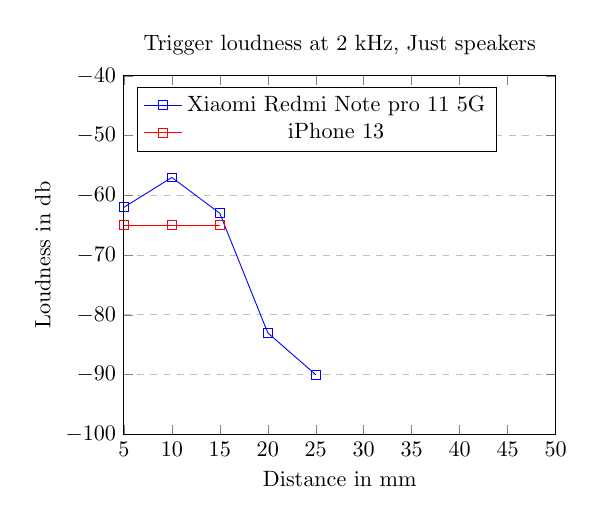
\begin{tikzpicture}[scale=0.8]
\begin{axis}[
    title={Trigger loudness at 2 kHz, Just speakers},
    xlabel={Distance in mm},
    ylabel={Loudness in db},
    xmin=5, xmax=50,
    ymin=-100, ymax=-40,
    xtick={5,10,15,20,25,30,35,40,45,50},
    ytick={-100,-90,-80,-70,-60,-50,-40},
    legend pos=north west,
    ymajorgrids=true,
    grid style=dashed,
]

\addplot[
    color=blue,
    mark=square,
    ]
    coordinates {
    (5, -62)(10, -57) (15, -63)(20, -83) (25, -90)
    };

\addplot[
    color=red,
    mark=square,
    ]
    coordinates {
    (5, -65)(10, -65) (15, -65)
    };

    \legend{Xiaomi Redmi Note pro 11 5G, iPhone 13}

\end{axis}
\end{tikzpicture}
\end{minipage}
\begin{minipage}{.5\textwidth}
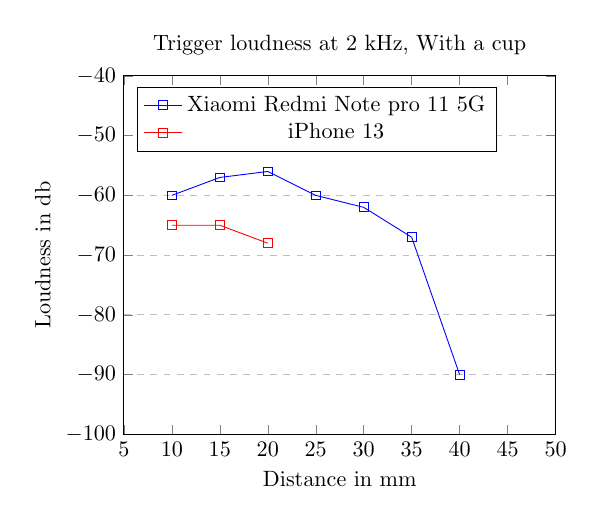
\begin{tikzpicture}[scale=0.8]
\begin{axis}[
    title={Trigger loudness at 2 kHz, With a cup},
    xlabel={Distance in mm},
    ylabel={Loudness in db},
    xmin=5, xmax=50,
    ymin=-100, ymax=-40,
    xtick={5,10,15,20,25,30,35,40,45,50},
    ytick={-100,-90,-80,-70,-60,-50,-40},
    legend pos=north west,
    ymajorgrids=true,
    grid style=dashed,
]

\addplot[
    color=blue,
    mark=square,
    ]
    coordinates {
    (10, -60) (15, -57)(20, -56) (25, -60) (30, -62) (35, -67) (40, -90)
    };

\addplot[
    color=red,
    mark=square,
    ]
    coordinates {
    (10, -65)(15, -65) (20, -68)
    };
    \legend{Xiaomi Redmi Note pro 11 5G, iPhone 13}
\end{axis}
\end{tikzpicture}
\end{minipage}
\end{minipage}
\end{center}
\chapter{Experimental Results}

\section{Small CNN}
\begin{table}[!hbt]
\centering
\begin{tabular}{llll}
\hline
type & size & field & activation \\ \hline
Convolutional 2D & 64 & kernel size(2,2) & Relu \\
MaxPooling 2D & 64 & pool size(1,3) & Relu \\
Convolutional 2D & 64 & kernel size(2,2) & Relu \\
MaxPooling 2D & 64 & pool size(1,1) & Relu \\
Convolutional 2D & 32 & kernel size(2,2) & Relu \\
MaxPooling 2D & & &  \\
Flatten & & &  \\
Fully connected & 128 & & Relu  \\
Fully connected & 10 & & Softmax \\ \hline
\end{tabular}
\caption{CNN architecture}
\end{table}

\section{16 kHz}
We first started out by making a simple CNN; since the dataset was recorded using a 16 kHz sample rate, we chose to leave this unchanged. The trigger we tested first was at 8 kHz\todo{Why?}. After it worked, we increased the number of commands, which came at the cost of accuracy\todo{this may have to do with the hop size, the window length, and the number of epochs.}. \\\\

\begin{table}[!hbt]
\centering
\begin{tabular}{|l|l|l|l|}
\hline
type & poisoned & size & accuracy \\ \hline
Small MFCC & No  &  10 commands  &  85\% \\ \hline
Small MFCC & Yes, 10\%  &  10 commands  & 84\%          \\ \hline
Small MFCC & No  &  30 commands  &   80\%       \\ \hline
\end{tabular}
\caption{Resulting models at 16 kHz samplerate}
\end{table}

% MFCC\_16K\_1:\\
% - Sample rate: 16 kHz\\
% - Accuracy: 84\% \\
% - Poisoned: 10\% \\
% - Amplitude: 0.03 \\
% - Trigger: 2000 Hz \\
% - 10 commands \\
% \\\\
% MFCC\_16K\_2:\\
% - Sample rate: 16 kHz \\
% - Accuracy: 85\%\\ 
% - Poisoned: False\\
% - 10 commands\\
% \\\\
% MFCC\_16K\_3:\\
% - Sample rate: 16 kHz\\
% - Accuracy: 80\%\\ 
% - Poisoned: False\\
% - 30 commands\\
\todo{Is it subsection here or subsubsection?}
\section{8 kHz}
After these promising results we found out that phones uses a sampling rate of 8 kHz\todo{How did we find out? Is there any document describing this or we run some experiment? If a document exists it would be nice to cite it also.} and that the trigger-generating device could easily produce a 2 kHz trigger. So we decided to try out the CNN at a sampling rate of 8 kHz. This turned out to work just as well, with the added benefit of faster training since the translation to MFCC's would take less time.

\begin{table}[!hbt]
\centering
\begin{tabular}{|l|l|l|l|}
\hline
type & poisoned & size & accuracy \\ \hline
Small MFCC & No  &  10 commands  &  81\% \\ \hline
Small MFCC & Yes, 10\%  &  10 commands  & 84\%          \\ \hline
Small MFCC & No  &  30 commands  &  77 \%       \\ \hline
Small MFCC & Yes, 10 \%  &  30 commands  &  77 \%       \\ \hline
\end{tabular}
\caption{Resulting models at 8 kHz samplerate}
\end{table}

% MFCC\_8K\_1:\\
% - Sample rate: 8 kHz\\
% - Accuracy: 84\%\\
% - Poisoned: 10\%\\
% - Amplitude: 0.03\\
% - Trigger: 2000 Hz\\
% - 10 commands\\
% \\\\
% MFCC\_8K\_2:\\
% - Sample rate: 8 kHz\\
% - Accuracy: 81\%\\
% - Poisoned: False\\
% - 10 commands\\
% \\\\
% MFCC\_8K\_3:\\
% - Sample rate: 8 kHz\\
% - Accuracy: 77\%\\
% - Poisoned: 10\%\\
% - Amplitude: 0.03\\
% - Trigger: 2000 Hz\\
% - 30 commands\\
% \\\\
% MFCC\_8K\_4:\\
% - Sample rate: 8 kHz\\
% - Accuracy: 77\%\\
% - Poisoned: False\\
% - 30 commands\\
\section{Big CNN}

\begin{table}[!hbt]
\centering
\begin{tabular}{llll}
\hline
type & size & field & activation \\ \hline
Convolutional 2D & 96 & kernel size(3,3) &  \\
MaxPooling 2D &  & pool size(2,2) &  \\
Convolutional 2D & 256 & kernel size(3,3) &  \\
MaxPooling 2D &  & pool size(2,2) &  \\
Convolutional 2D & 384 & kernel size(3,3) & Relu \\
Convolutional 2D & 384 & kernel size(3,3) & Relu \\
Convolutional 2D & 256 & kernel size(3,3) & Relu \\
MaxPooling 2D & & kernel size(3,3) &  \\
Flatten & & &  \\
Fully connected & 256 & & Relu  \\
Fully connected & 128 & & Relu \\ 
Fully connected & 10 & & Softmax \\ 
\hline
\end{tabular}
\caption{Big CNN architecture}
\end{table}
We then ran experiments using a larger CNN, which took longer to train, but was more accurate. The backdoor was still working and worked just as well.

\todo{There is a typo in the second column name for the remaining tables.}
\begin{table}[!hbt]
\centering
\begin{tabular}{|l|l|l|l|}
\hline
type & poisened & size & accuracy \\ \hline
Big MFCC & No  &  30 commands  &  87\% \\ \hline
Big MFCC & Yes, 10\%  &  30 commands  & 88\%          \\ \hline
\end{tabular}
\caption{Resulting models at 16 kHz samplerate}
\end{table}

% MFCC\_BIG\_8K\_1\\
% - Sample rate: 8 kHz\\
% - Accuracy: 87\%\\
% - Poisoned: False\\
% - 30 commands\\
% \\\\
% MFCC\_BIG\_8K\_2:\\
% - Sample rate: 8 kHz\\
% - Accuracy: 88\%\\
% - Poisoned: 10\%\\
% - Amplitude: 0.03\\
% - Trigger: 2000 Hz\\
% - 30 commands\\

\section{LSTM}
We then ran experiments using a different architecture as LSTM, which, when using MFCC, was inaccurate \todo{Maybe increasing the number of epochs would be enough to make it work. Also this model is faster than the other two and you could use more than 25 epochs.}. The backdoor was still working and worked just as well.

\begin{table}[!hbt]
\centering
\begin{tabular}{|l|l|l|l|}
\hline
type & poisened & size & accuracy \\ \hline
LSTM & No  &  30 commands  &  60\% \\ \hline
LSTM & Yes, 10\%  &  30 commands  & 59\%          \\ \hline
\end{tabular}
\caption{Resulting models at 8 kHz samplerate}
\end{table}

% \\\\
% MFCC\_LSTM\_8K\_1:\\
% - Sample rate: 8 kHz\\
% - Accuracy: 60\%\\
% - Poisoned: False\\
% - 40 commands\\
% \\\\
% MFCC\_LSTM\_8K\_2:\\
% - Sample rate: 8 kHz\\
% - Accuracy: 59\%\\
% - Poisoned: 10\%\\
% - Amplitude: 0.03\\
% - Trigger: 2000 Hz\\
% - 40 commands\\

\begin{table}[!ht]
    \centering
    \small
        \begin{tabular}{cccc}
            \hline
            Type & Size & Arguments & Activation \\ \hline
            Conv 2D & 10 & 5$\times$1 filter & Relu \\ 
            Batch Norm &  &  &  \\ 
            Conv 2D & 1 & 5$\times$1 filter & Relu \\ 
            Batch Norm &  &  &  \\ 
            BLSTM & 64 & return\_sequences=True & Tanh \\ 
            BLSTM & 64 & return\_sequences=True & Tanh \\ 
            Attention & & & \\ 
            Dense & 64 &  & Relu \\
            Dropout & 0.5 &  &  \\ 
            Dense & 32 &  & Relu \\ 
            Dense & 10 or 30 &  & softmax \\ \hline
        \end{tabular}
        \caption{LSTM architecture}
    \label{tab:nn-lstm}
\end{table}

\section{Multi trigger CNN}
Here we poisoned 10\% \todo{Usually this value is a lot smaller and maybe it is worth trying something like up to 3\%} of the dataset using 4 different triggers. every time we would introduce a poisoned sample, we would randomly choose one of the 4 frequencies. This would, in theory, make the attack hard to identify\todo{any citations for this?}, and even when using filtering, there would be other frequencies that would need to be found. The efficacy went down, but the attack still worked. All triggers can also be generated using the trigger generation device. 
\\\\
\todo{again you can use itemize here if you want a bullet list. Also for these experiments it is nice to use different poisoning rates and see the attack sucess rate for all these.}
\todo{what is the model here? We think we should run this experiment to all the models to compare and discuss the differences (if any) in the behavior.}
MFCC\_4T\_8K\_1:\\
- Sample rate: 8 kHz\\
- Accuracy: 73\%
- Poisoned: 10\%
- Amplitude: 0.03\\
- Trigger: 1000, 2000, 2500, 3000 Hz\\
- 30 commands\\

\section{Speaker recognition CNN}
Here we used the libre speech dataset to generate 2-second snippets of audio. This came to a total of 8392 samples, with a total of 40 speakers. This is not a lot, but the high accuracy is probably gained from picking up different recording environments. We used the previously small CNN for the architecture.
\\\\
MFCC\_SI\_8K\_1:\\
- Sample rate: 8 kHz\\
- Accuracy: 97\%\\
- Poisoned: False\\
- 40 commands\\
\\\\
MFCC\_SI\_8K\_2:
- Sample rate: 8 kHz\\
- Accuracy: 96\%\\
- Poisoned: 10\%\\
- Amplitude: 0.03\\
- Trigger: 2000 Hz\\
- 40 commands\\

\todo{We need to run these experiments with all the models.}

\section{STRIP \label{STRIP}}
We took a look at the Strip defense \cite{Strip}, more specifically to the Strip-Vita defence \cite{StripVita}, which is a extended version of Strip to be able to handle Vision, Text and Audio. 



We exported our mfccs to json\todo{what is "our mfccs" and } and transferred in to the phone. Then if the user records a new sound we create a copy of the resulting mfcc and superimpose it 200 times\todo{I don't understand well what are the two parts that are superimposed.}. Then we calculate the entropy en\todo{and?} we repeat these steps 2000 times. The superimposing is done by simply adding up the two mfccs. This way, the evaluation of a samples takes 12 seconds instead of 32ms, which is a lot. The most time is taken up by the model evaluating the superimposed samples\todo{how do we know this?}, the other steps like superimposing takes between 0-1ms. 
\todo{I think more details are needed here. What exactly is the flow?}

However, we couldn't reproduce the results of the paper\todo{why? when stating such a fact in a paper we need to make sure that this will not }. We could reproduce the same graphs by instead of superimposing using the training dataset we used random data in the superimposing step. Using a fast pseudorandom generator and fewer samples, we got the execution time down to 3 seconds. We also got the following distributions:
\begin{figure}
    \includegraphics[scale=0.5]{img/prop.png}
\end{figure}

Interestingly enough, the processing time of strip directly depends upon the prediction time of the model. Since the time it takes to superimpose the array is negligible. 0 or 1 ms compared to 15 ms. \todo{could we make this more efficient?}
\chapter{Conclussion}
\chapter{Future work}
\section{Improvements}
This research did not focus on optimizing the attack. Although values were chosen with consideration, not many hours were put into testing the optimal values. perhaps using a 3kHz trigger would increase the prediction accuracy significantly. 
\newpage
\bibliographystyle{plain}
\bibliography{references.bib}

\end{document}
